\documentclass[11pt,a4paper]{article}
\usepackage[margin=1in]{geometry}
\usepackage{graphicx}
\usepackage{booktabs}
\usepackage{longtable}
\usepackage{caption}
\usepackage{hyperref}
\usepackage{array}
\usepackage{float}
\usepackage{listings}
\usepackage{xcolor}
\usepackage{amsmath}

\captionsetup{font=small,labelfont=bf}

\lstset{
  language=Python,
  basicstyle=\ttfamily\small,
  keywordstyle=\color{blue}\bfseries,
  commentstyle=\color{gray},
  stringstyle=\color{red},
  breaklines=true,
  showstringspaces=false,
  frame=single,
  numbers=left,
  numberstyle=\tiny,
  captionpos=b
}

\title{Experiment 5: Perceptron Learning Algorithm (PLA) \\ \large One-vs-Rest Multi-class Classification}
\author{Prepared by: \textbf{Sreeram GM} \\
Course / Lab: Experiment 5}
\date{\today}

\begin{document}
\maketitle
\tableofcontents
\bigskip

\section{Aim}
Implement the Perceptron Learning Algorithm (PLA) as a one-vs-rest multi-class classifier for the image dataset, perform hyperparameter search, evaluate the best model on a held-out test set, and present results (metrics, confusion matrix, ROC, training-error curve).

\section{Dataset}
\begin{itemize}
  \item Dataset root (Colab / Google Drive): \texttt{/content/drive/MyDrive/colabdata/dataset}
  \item Contents:
    \begin{itemize}
      \item \texttt{Img/} : folder containing image files.
      \item \texttt{*.csv} : CSV file mapping image filenames to labels.
    \end{itemize}
  \item Summary (from experiment run):
    \begin{itemize}
      \item Number of classes: \textbf{62}
      \item Train samples: \textbf{2728}
      \item Test samples: \textbf{682}
    \end{itemize}
\end{itemize}

\section{Preprocessing}
\begin{enumerate}
  \item Mount Google Drive in Colab and locate dataset folder.
  \item Load CSV mapping filenames to labels; auto-detect filename and label columns when possible.
  \item For each image:
    \begin{itemize}
      \item Convert to grayscale (PIL `L`).
      \item Resize to \textbf{28$\times$28}.
      \item Normalize pixel values to $[0,1]$.
      \item Flatten to a vector of length $784$.
    \end{itemize}
  \item Use \texttt{LabelEncoder} to convert labels into integer class indices.
  \item Use stratified train/test split (80\% train, 20\% test). During hyperparameter search, use an internal validation split from train.
\end{enumerate}

\section{Implementation}
Below are the key code sections used in the experiment. The full code is included in the appendix.

\subsection{Mounting and CSV / Image loading}
\begin{lstlisting}[caption={Mount Drive and auto-detect CSV + load filenames}]
from google.colab import drive
drive.mount('/content/drive')

DATASET_ROOT = '/content/drive/MyDrive/colabdata/dataset'
IMG_FOLDER = DATASET_ROOT + '/Img'

# find CSV file in dataset root
def find_csv_file(dataset_root):
    candidates = [f for f in os.listdir(dataset_root) if f.lower().endswith('.csv')]
    if not candidates:
        raise FileNotFoundError(f"No CSV file found in {dataset_root}. Place CSV in that folder.")
    return os.path.join(dataset_root, candidates[0])

CSV_PATH = find_csv_file(DATASET_ROOT)
df = pd.read_csv(CSV_PATH).dropna().reset_index(drop=True)

# auto-detect filename & label columns
possible_file_cols = ['filename','file','image','img','path','image_path','file_name','File']
possible_label_cols = ['label','class','target','y','label_name','Label']
file_col = None
label_col = None
for c in df.columns:
    low = c.lower()
    if low in possible_file_cols or any(p in low for p in possible_file_cols):
        file_col = c
    if low in possible_label_cols or any(p in low for p in possible_label_cols):
        label_col = c
if file_col is None: file_col = df.columns[0]
if label_col is None: label_col = df.columns[1] if len(df.columns)>1 else df.columns[0]
print("Detected file column:", file_col)
print("Detected label column:", label_col)
\end{lstlisting}

\subsection{Preprocessing function and dataset build}
\begin{lstlisting}[caption={Image preprocessing and building X,y arrays}]
from PIL import Image
import numpy as np

def load_and_preprocess(img_path, size=(28,28), as_gray=True):
    img = Image.open(img_path)
    if as_gray:
        img = img.convert('L')
    img = img.resize(size, Image.BILINEAR)
    arr = np.asarray(img, dtype=np.float32)/255.0
    return arr.flatten()

# Resolve paths and build lists
image_paths = []
labels = []
missing_files = []
for idx, row in df.iterrows():
    fname = str(row[file_col])
    full_path = fname
    if not os.path.isabs(full_path):
        p1 = os.path.join(IMG_FOLDER, fname)
        p2 = os.path.join(IMG_FOLDER, os.path.basename(fname))
        if os.path.exists(p1): full_path = p1
        elif os.path.exists(p2): full_path = p2
        else:
            p3 = os.path.join(DATASET_ROOT, fname)
            if os.path.exists(p3): full_path = p3
            else:
                missing_files.append(fname)
                continue
    image_paths.append(full_path)
    labels.append(row[label_col])

# load images (can be slow)
X_list = []
for p in tqdm(image_paths):
    X_list.append(load_and_preprocess(p, size=(28,28)))
X = np.vstack(X_list)
y = np.array(labels)
\end{lstlisting}

\subsection{Label encoding and splitting}
\begin{lstlisting}[caption={Label encoding and train/test split}]
from sklearn.preprocessing import LabelEncoder
from sklearn.model_selection import train_test_split

le = LabelEncoder()
y_enc = le.fit_transform(y)
classes = le.classes_
n_classes = len(classes)

X_train, X_test, y_train_idx, y_test_idx = train_test_split(
    X, y_enc, test_size=0.2, stratify=y_enc, random_state=42)
\end{lstlisting}

\subsection{PLA (One-vs-Rest) implementation}
\begin{lstlisting}[caption={Perceptron PLA class and OvR training}]
class PerceptronPLA:
    def __init__(self, n_features, lr=1.0):
        self.lr = lr
        self.w = np.zeros(n_features + 1, dtype=np.float32)  # include bias

    def predict_raw(self, X):
        Xb = np.hstack([X, np.ones((X.shape[0],1), dtype=np.float32)])
        return Xb.dot(self.w)

    def predict(self, X):
        return np.where(self.predict_raw(X) >= 0, 1, -1)

    def fit(self, X, y, epochs=10, shuffle=True, verbose=False):
        Xb = np.hstack([X, np.ones((X.shape[0],1), dtype=np.float32)])
        n = X.shape[0]
        history = []
        for ep in range(epochs):
            errors = 0
            indices = np.arange(n)
            if shuffle: np.random.shuffle(indices)
            for i in indices:
                xi = Xb[i]; yi = y[i]
                pred = 1 if xi.dot(self.w) >= 0 else -1
                if pred != yi:
                    self.w += self.lr * yi * xi
                    errors += 1
            history.append(errors / n)
        return history

def train_ovr_pla(X_train, y_train, lr=1.0, epochs=20):
    n_features = X_train.shape[1]
    models = {}
    history = {}
    for c_idx, c_label in enumerate(classes):
        y_bin = np.where(y_train == c_idx, 1, -1)
        p = PerceptronPLA(n_features, lr=lr)
        hist = p.fit(X_train, y_bin, epochs=epochs)
        models[c_idx] = p
        history[c_idx] = hist
    return models, history
\end{lstlisting}

\subsection{Hyperparameter search (grid) and retraining}
\begin{lstlisting}[caption={Grid search over LR and epochs; retrain best on full train}]
# grid
lr_values = [1.0, 0.1, 0.01]
epoch_values = [10, 20, 50]

best_acc = 0.0
best_params = None
best_models = None
best_history = None

search_X_tr, search_X_val, search_y_tr, search_y_val = train_test_split(
    X_train, y_train_idx, test_size=0.2, stratify=y_train_idx, random_state=42)

for lr in lr_values:
    for ep in epoch_values:
        candidate_models, candidate_hist = train_ovr_pla(search_X_tr, search_y_tr, lr=lr, epochs=ep)
        # validation predictions
        def ovr_predict_local(models, X_input):
            n_samples = X_input.shape[0]
            scores_loc = np.zeros((n_samples, len(models)), dtype=np.float32)
            for c_idx, m in models.items():
                scores_loc[:, c_idx] = m.predict_raw(X_input)
            preds_loc = np.argmax(scores_loc, axis=1)
            return preds_loc
        val_preds = ovr_predict_local(candidate_models, search_X_val)
        acc = accuracy_score(search_y_val, val_preds)
        if acc > best_acc:
            best_acc = acc
            best_params = (lr, ep)
            best_models = candidate_models
            best_history = candidate_hist

# retrain on full X_train with best params
best_lr, best_ep = best_params
models, hist = train_ovr_pla(X_train, y_train_idx, lr=best_lr, epochs=best_ep)
\end{lstlisting}

\subsection{Evaluation and saving}
\begin{lstlisting}[caption={Prediction, metrics, plots, save weights}]
def ovr_predict(models, X):
    n = X.shape[0]
    scores = np.zeros((n, len(models)), dtype=np.float32)
    for c_idx, model in models.items():
        scores[:, c_idx] = model.predict_raw(X)
    preds = np.argmax(scores, axis=1)
    return preds, scores

y_pred_idx, raw_scores_test = ovr_predict(models, X_test)

# metrics
acc = accuracy_score(y_test_idx, y_pred_idx)
prec, rec, f1, _ = precision_recall_fscore_support(y_test_idx, y_pred_idx, average='macro', zero_division=0)

# save models
with open('/content/pla_ovr_models.pkl','wb') as f:
    pickle.dump({'best_params':best_params,'models':{c:m.w for c,m in models.items()}, 'label_encoder':le}, f)
\end{lstlisting}

\section{Hyperparameter Search and Best Configuration}
\begin{itemize}
  \item Grid searched: Learning rates = \{1.0, 0.1, 0.01\}; Epochs = \{10, 20, 50\}.
  \item Best hyperparameters: \textbf{learning rate = 0.1, epochs = 50}.
  \item Best validation accuracy (internal validation): \textbf{0.1978}.
\end{itemize}

\section{Results}
\subsection{Overall summary}
\begin{itemize}
  \item Number of classes: \textbf{62}
  \item Train samples: \textbf{2728}
  \item Test samples: \textbf{682}
  \item Best LR, epochs: \textbf{(0.1, 50)}
  \item Validation accuracy (best): \textbf{0.1978}
  \item Accuracy (test): \textbf{0.1833}
  \item Macro F1: \textbf{0.1674}
\end{itemize}

\subsection{Per-class precision / recall / f1}
\small
\begin{longtable}{@{}l c c c@{}}
\caption{Per-class metrics (test set)}\\
\toprule
\textbf{class\_label} & \textbf{precision} & \textbf{recall} & \textbf{f1} \\
\midrule
\endfirsthead
\toprule
\textbf{class\_label} & \textbf{precision} & \textbf{recall} & \textbf{f1} \\
\midrule
\endhead
\bottomrule
\endfoot
0  & 0.214286 & 0.272727 & 0.240000 \\
1  & 0.083969 & 1.000000 & 0.154930 \\
2  & 1.000000 & 0.090909 & 0.166667 \\
3  & 0.666667 & 0.181818 & 0.285714 \\
4  & 0.000000 & 0.000000 & 0.000000 \\
5  & 0.500000 & 0.090909 & 0.153846 \\
6  & 0.000000 & 0.000000 & 0.000000 \\
7  & 0.000000 & 0.000000 & 0.000000 \\
8  & 0.666667 & 0.181818 & 0.285714 \\
9  & 0.000000 & 0.000000 & 0.000000 \\
A  & 0.000000 & 0.000000 & 0.000000 \\
B  & 1.000000 & 0.272727 & 0.428571 \\
C  & 0.250000 & 0.727273 & 0.372093 \\
D  & 1.000000 & 0.090909 & 0.166667 \\
E  & 0.375000 & 0.272727 & 0.315789 \\
F  & 0.000000 & 0.000000 & 0.000000 \\
G  & 0.444444 & 0.363636 & 0.400000 \\
H  & 1.000000 & 0.090909 & 0.166667 \\
I  & 0.000000 & 0.000000 & 0.000000 \\
J  & 0.375000 & 0.545455 & 0.444444 \\
K  & 0.000000 & 0.000000 & 0.000000 \\
L  & 1.000000 & 0.363636 & 0.533333 \\
M  & 0.666667 & 0.363636 & 0.470588 \\
N  & 1.000000 & 0.090909 & 0.166667 \\
O  & 0.166667 & 0.090909 & 0.117647 \\
P  & 0.470588 & 0.727273 & 0.571429 \\
Q  & 0.291667 & 0.636364 & 0.400000 \\
R  & 1.000000 & 0.090909 & 0.166667 \\
S  & 0.000000 & 0.000000 & 0.000000 \\
T  & 0.454545 & 0.454545 & 0.454545 \\
U  & 0.600000 & 0.272727 & 0.375000 \\
V  & 0.363636 & 0.363636 & 0.363636 \\
W  & 0.000000 & 0.000000 & 0.000000 \\
X  & 1.000000 & 0.181818 & 0.307692 \\
Y  & 0.000000 & 0.000000 & 0.000000 \\
Z  & 0.500000 & 0.090909 & 0.153846 \\
a  & 1.000000 & 0.090909 & 0.166667 \\
b  & 0.000000 & 0.000000 & 0.000000 \\
c  & 0.333333 & 0.181818 & 0.235294 \\
d  & 0.133333 & 0.181818 & 0.153846 \\
e  & 0.076923 & 0.090909 & 0.083333 \\
f  & 0.000000 & 0.000000 & 0.000000 \\
g  & 0.111111 & 0.272727 & 0.157895 \\
h  & 0.045455 & 0.272727 & 0.077922 \\
i  & 0.333333 & 0.181818 & 0.235294 \\
j  & 0.200000 & 0.090909 & 0.125000 \\
k  & 0.014925 & 0.090909 & 0.025641 \\
l  & 0.000000 & 0.000000 & 0.000000 \\
m  & 1.000000 & 0.090909 & 0.166667 \\
n  & 0.000000 & 0.000000 & 0.000000 \\
o  & 0.000000 & 0.000000 & 0.000000 \\
p  & 0.571429 & 0.363636 & 0.444444 \\
q  & 0.114286 & 0.727273 & 0.197531 \\
r  & 0.153846 & 0.363636 & 0.216216 \\
s  & 0.130435 & 0.272727 & 0.176471 \\
t  & 0.083333 & 0.090909 & 0.086957 \\
u  & 0.000000 & 0.000000 & 0.000000 \\
v  & 0.000000 & 0.000000 & 0.000000 \\
w  & 0.000000 & 0.000000 & 0.000000 \\
x  & 0.000000 & 0.000000 & 0.000000 \\
y  & 1.000000 & 0.090909 & 0.166667 \\
z  & 0.000000 & 0.000000 & 0.000000 \\
\end{longtable}
\normalsize

\subsection{Figures (placeholders)}
\begin{figure}[H]
  \centering
  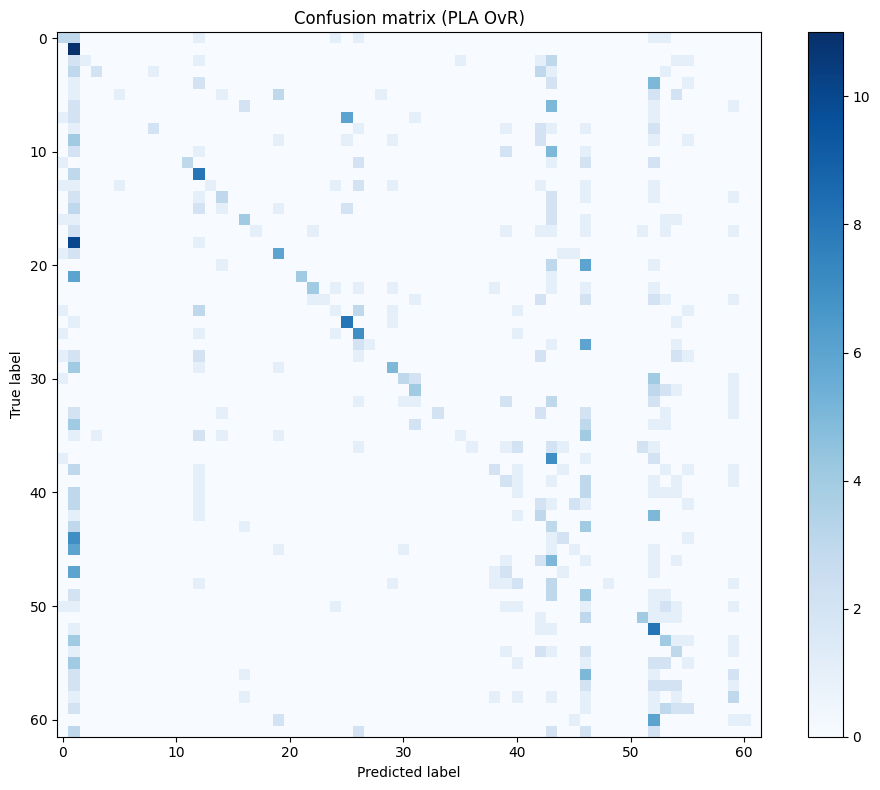
\includegraphics[width=0.7\linewidth]{PLA_images/cn_matrix.png}
  \caption{Confusion matrix (replace with actual image path).}
  \label{fig:confmat}
\end{figure}

\begin{figure}[H]
  \centering
  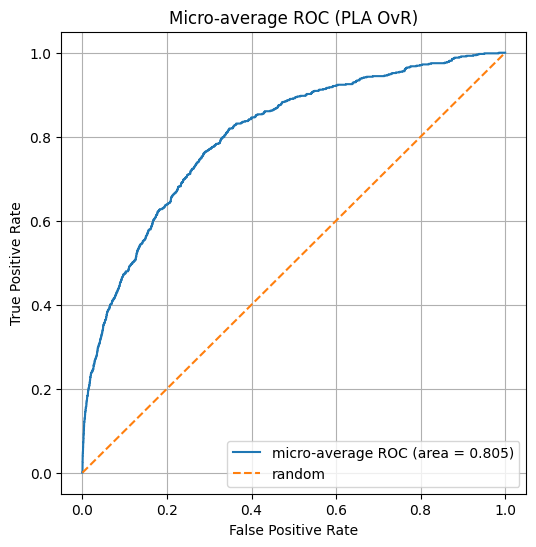
\includegraphics[width=0.7\linewidth]{PLA_images/roc.png}
  \caption{Micro-average ROC curve (replace with actual image path).}
  \label{fig:roc}
\end{figure}

\begin{figure}[H]
  \centering
  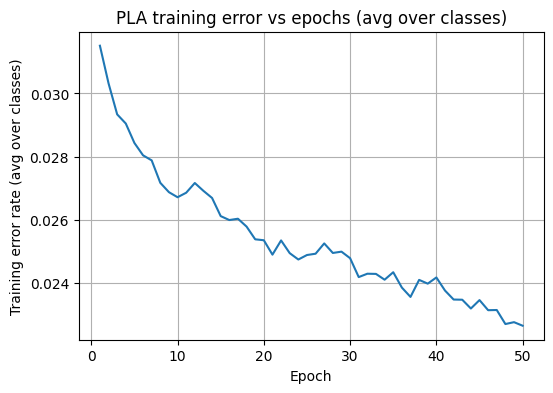
\includegraphics[width=0.7\linewidth]{PLA_images/error.png}
  \caption{Training error vs epochs (average over classes).}
  \label{fig:trainerr}
\end{figure}

\section{Discussion}
\begin{itemize}
  \item Test accuracy is low (about 18.33\%) and macro F1 is 0.1674. This indicates the dataset is challenging for PLA, likely due to:
    \begin{itemize}
      \item Large number of classes (62) with limited samples per class.
      \item High intra-class variability and possible class imbalance.
      \item PLA is a linear classifier and may not capture complex patterns in image data.
    \end{itemize}
  \item Some classes have very high precision but very low recall (or vice versa), indicating the classifier is biased / sparse in predictions for those classes.
  \item Consider stronger models (MLP/CNN), data augmentation, feature extraction, or dimensionality reduction for improved performance.
\end{itemize}

\section{Conclusion}
The PLA (OvR) baseline was implemented and tuned with grid search. While it works end-to-end and provides interpretable per-class metrics, its performance on this image classification task is limited. Use the results as a baseline for comparison with MLP/CNN models.

\appendix

\end{document}
